% Insert inside the manuscript's Results section.
\subsection*{Ingredient similarity is structured by cuisine}
The ingredient-based recipe network contained 26,727 recipes, 309,019 weighted edges, and 345 isolated recipes. Cuisine labels were not used to construct the network. Nevertheless, 63.0\% of total edge weight connected recipes assigned to the same cuisine, compared with 17.1\% under shuffled cuisine labels (95\% permutation reference interval, 16.9--17.4\%; $P_{\mathrm{perm}}=0.005$ from 199 shuffles). Every cuisine had a higher within-cuisine share than expected from its frequency in the dataset (Fig.~\ref{fig:network-structure}A). Community detection, also performed without cuisine labels, showed moderate alignment with the labels (adjusted mutual information $=0.367$, $P_{\mathrm{perm}}=0.005$). The within-cuisine share remained between 62.7\% and 64.1\% when the minimum Jaccard similarity was varied from 0.12 to 0.24.

Under the stricter recipe--ingredient randomization, which preserved recipe lengths and ingredient frequencies within each cuisine, the median within-cuisine weight share was 59.3\% (central 95\% randomization range, 58.7--59.8\%; Fig.~\ref{fig:recipe-null}A). The observed 63.0\% exceeded all 49 randomized networks ($P_{\mathrm{MC}}=0.02$, one-sided). Thus cuisine-specific ingredient frequencies account for much of the contrast with label shuffling, while ingredient co-occurrence within recipes adds a smaller residual of 3.7 percentage points. A five-run check with twice as many ingredient trades gave a similar median of 59.3\%.

We then recovered the original Food.com course tags and restricted ingredient trades to recipes sharing both cuisine and a primary dish type. A course tag was available for 25,099 of 26,727 recipes; the others formed an other/unclear group. This stronger null gave a median within-cuisine weight share of 59.0\% (central 95\% range, 58.7--59.4\%; Fig.~\ref{fig:recipe-null}A), close to the cuisine-only null. The observed 63.0\% again exceeded all 49 randomizations ($P_{\mathrm{MC}}=0.02$). Five-run diagnostics with twice as many trades or with complete course-tag combinations rather than primary types gave medians of 59.1\% in both cases. Preserving these broad dish types therefore did not remove the residual in this network.

The residual persisted after excluding 1,307 recipes explicitly named as sweets or drinks (65.3\% observed versus 59.7\% randomized median) and after excluding edges with Jaccard similarity at least 0.75 (62.9\% versus 59.3\%). Removing the original dessert-rich mixed community 76 increased the gap to 67.7\% versus 61.2\%; because that community was detected in the observed graph, this is a descriptive sensitivity check rather than an independent test.

\subsection*{Cross-cuisine links are unevenly distributed}
We compared the weight assigned to each cuisine pair as a fraction of all cross-cuisine edge weight, using 999 shuffled-label networks as a reference (Fig.~\ref{fig:network-structure}B). Chinese--Japanese links accounted for 4.38\% of observed cross-cuisine weight versus 0.51\% in the null mean (8.54-fold). The corresponding values were 6.85\% versus 1.43\% for Greek--Middle Eastern (4.79-fold) and 14.56\% versus 5.33\% for French--Italian (2.73-fold). These are descriptive examples chosen after inspecting the network, not formal tests of particular cuisine pairs. The statistic measures which pairs account for a relatively large share of the observed links between cuisines; it does not imply more links than expected under unrestricted random labeling. In a spot check of selected high-similarity edges, tzatziki and Turkish cacik, as well as French pistou and Italian pesto, illustrated related ingredient patterns. The same review identified ambiguous cuisine tags and nearly identical ingredient lists, which limit interpretations of individual links.

The recipe--ingredient null changes the interpretation of these selected pair affinities (Fig.~\ref{fig:recipe-null}B--D). Chinese--Japanese links made up 4.38\% of observed cross-cuisine weight, below the randomized median of 5.00\%; their large label-shuffle affinity is therefore compatible with cuisine-specific ingredient popularity. Greek--Middle Eastern links made up 6.85\%, above the randomized median of 6.28\% and all 49 replicates. French--Italian links made up 14.56\%, within the central 95\% randomization range of 13.64--14.73\%. These pair comparisons are exploratory because the pairs were chosen from the observed network.

Conditioning additionally on primary dish type gave medians of 4.62\%, 6.13\%, and 14.37\% for Chinese--Japanese, Greek--Middle Eastern, and French--Italian shares, respectively (Fig.~\ref{fig:recipe-null}B--D). The first observed share remained below all 49 randomizations, the second above all 49, and the third inside its central randomization range. This pattern was robust to broad dish-type composition, while the pair-level findings remain exploratory.

\begin{figure*}[t!]
\centering
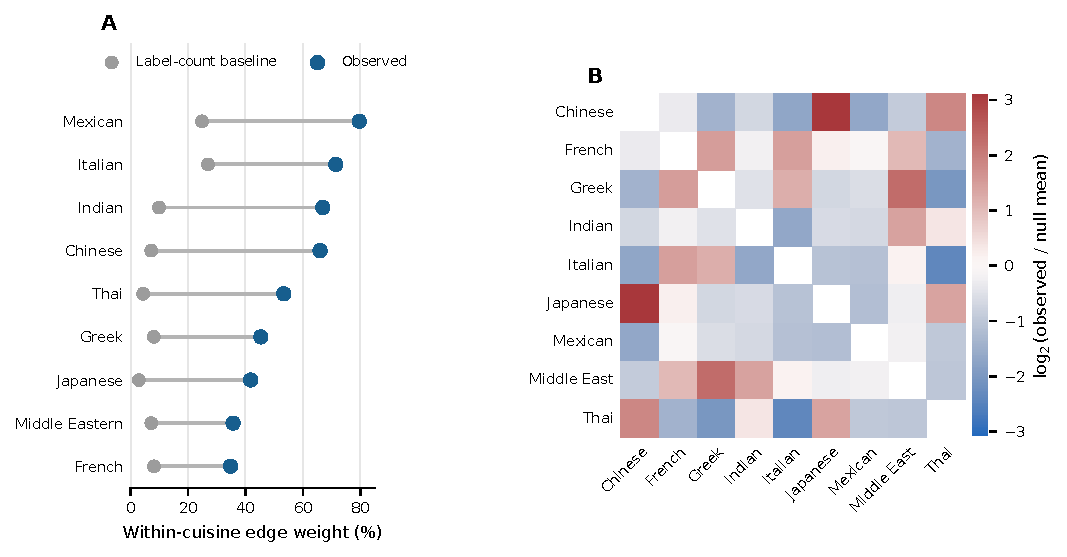
\includegraphics[width=17.8cm]{pnas_network/pnas_network_figure.pdf}
\caption{Cuisine structure in the ingredient-based recipe network. (A) For each cuisine, blue points show the observed fraction of incident edge weight connected to recipes with the same label. Gray points show the label-count baseline $(n_c-1)/(n-1)$; lines connect the two values. (B) Relative affinity of cuisine pairs among cross-cuisine edges, shown as $\log_2$ of the observed share divided by the mean share from 999 fixed-graph label permutations. Red indicates a larger relative share and blue a smaller one; diagonal cells are undefined. The graph contains 26,727 recipes and 309,019 edges.}
\label{fig:network-structure}
\end{figure*}

\begin{figure*}[t!]
\centering
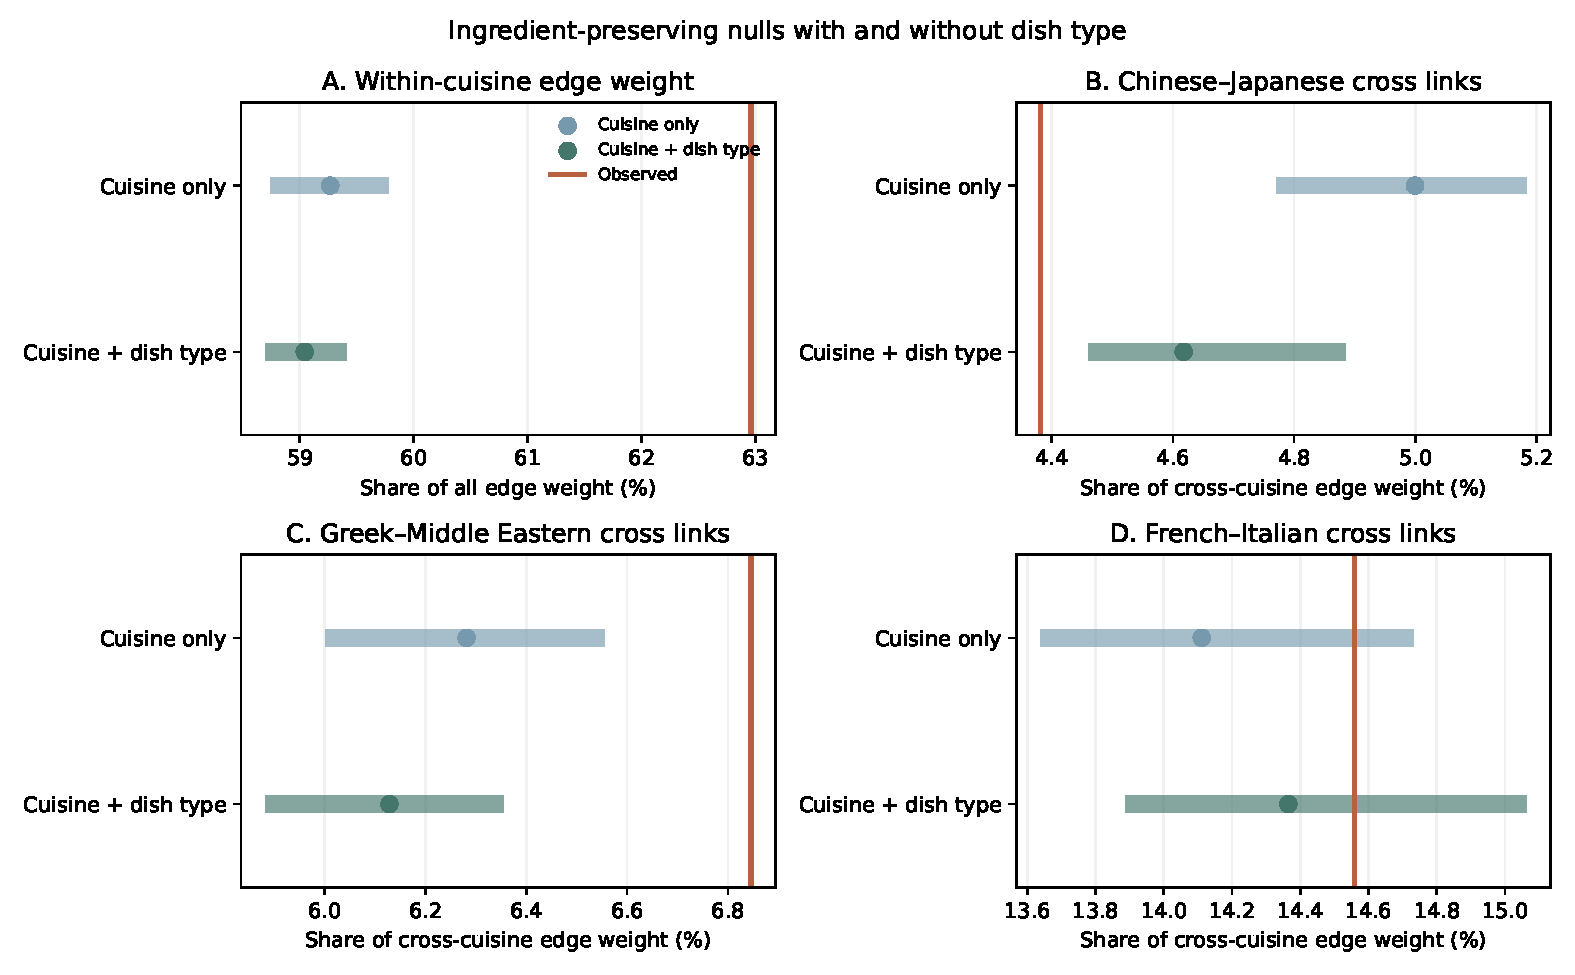
\includegraphics[width=17.8cm]{pnas_network/pnas_tagged_null_figure.pdf}
\caption{Ingredient-level null distributions after rebuilding the recipe network. Points show medians and thick bars the central 95\% ranges of 49 randomizations each, exchanging ingredients within cuisine (blue) or within cuisine and primary dish type (green). Both preserve each recipe's retained-ingredient count and the ingredient frequencies in their respective strata. Red lines show the observed network. (A) Within-cuisine share of total edge weight. (B--D) Selected cuisine-pair shares of cross-cuisine edge weight; pair selection was exploratory.}
\label{fig:recipe-null}
\end{figure*}
